\mode<presentation>
{
  \usetheme{CambridgeUS}
  \usecolortheme{whale}
  \usecolortheme{lily}

  \setbeamercovered{transparent}
  \usefonttheme[onlymath]{serif}
}

\title[\LaplaceTransformReviewShortName] % (optional, use only with long paper titles)
{\course: \LaplaceTransformReviewName\license}

\subtitle
{Lecture \LaplaceTransformReviewNumber} % (optional)


\begin{document}

\begin{frame}
  \titlepage
\end{frame}

\mode<article>{
\maketitle
\tableofcontents
}

%\mode<presentation>{
%\begin{frame}{Outline}
%  \tableofcontents
%  % You might wish to add the option [pausesections]
%\end{frame}}

\section{Pre-requisite Material}
This lecture assumes that the reader is familiar with the following material:
\begin{itemize}
\item Differential equations
\item Integration
\item Complex numbers, including Euler's Formula
\end{itemize}

\section{Motivation}

We have seen in previous lectures that differential equations model dynamic systems. We will be using these equations to predict how systems will respond to inputs, thus control system design requires simple methods for solving these equations! Laplace Transforms are a useful tool that allows us to systematically solve linear time invariant (LTI) equations for arbitrary inputs, easily combine coupled differential equations, as well as allow us to use block diagrams to represent systems that are made up of smaller subsystems.

Laplace Transforms may initially seem strange and arbitrary, but we should recognize that we have already used transformations before in mathematics. For example, consider the transformation between rectangular form and polar form for complex numbers. 

\begin{frame}{Complex Representation Transform}
\[
\begin{matrix} \mbox{Rectangular Form} & \mbox{Polar Form} \\
s=a+jb & s=r\angle \theta
\end{matrix}
\]
Given a complex number represented in rectangular form, we can {\em transform} it to polar form (and vice-versa)
\[
(a,b) \leftrightarrow (r,\theta)
\]
\end{frame}\vspace{-10pt}

Thus, the pair $(a,b)$ and the pair $(r,\theta)$ represent the {\em same} complex number, but they do it in different ways that might be more useful in some contexts. For example, multiplication of complex numbers is much easier in polar form than it is in rectangular form, especially if we are multiplying many complex numbers together. 

Laplace Transforms take a function of a real variable, $t$, and transform it to a function of a complex variable, $s$. These will represent the {\em same} function of time, but we will see that solving differential equations is easier with the second representation. 

\section{Laplace Transform Definition}

\begin{frame}{Laplace Transform Definition}
\begin{center}
Let $f(t)$ be a function of time defined for $t>0$. The one-sided Laplace Transform of $f(t)$ is defined to be
\end{center}
\[
\boxed{F(s) := \mathcal{L}[f(t)] := \int_{0^{-}}^{\infty} f(t)e^{-st}dt}
\]
\begin{itemize}
\item $0^{-}$ is shorthand for the lower limit approaching $0$ from the left (always negative)
\item The Laplace Transform exists if the integral converges for {\em any} value of $s$
\begin{itemize}
\item Region of convergence is not as important for ``one-sided'' Laplace transforms
\end{itemize}
\end{itemize}
\end{frame}

\begin{frame}{Important facts you should already know}
\begin{itemize}
\item Complex Exponentials (Euler's Formula): $e^{j\theta} = \cos(\theta) + j \sin(\theta)$.
\item Differentiation and integration with $s$ as a complex number: 
\[
\frac{d}{dt}e^{st} = s e^{st}
\]
\[
\int_{a}^{b} e^{st}dt = \left.\frac{1}{s} e^{st}\right|_{a}^{b}
\]
\end{itemize}
\end{frame}
For derivations, see the appendix.

\subsection{Finding Laplace Transforms using the definition}

\begin{example}
Find the one-sided Laplace Transform of the function
\[
f(t)= 3
\]
\textbf{Solution: } Plug the function into the Laplace Transform definition
\begin{align*}
F(s) &= \int_{0^{-}}^{\infty} 3e^{-st}dt \\
&= \left.\frac{1}{-s}3e^{-st}\right|_{0^{-}}^{\infty}\\
& = \frac{3}{-s}\left[\lim_{t\rightarrow \infty}e^{-st} - \lim_{t\rightarrow 0^{-}}e^{-st} \right]
\end{align*}
\begin{itemize}
\item Laplace Transform is defined if it converges for {\em any} value of $s$. 
\begin{itemize}
\item Second limit converges to 1 for all values of s
\item First limit converges to zero if the real part of $s$ is greater than zero
\end{itemize}
\begin{align*}
F(s)&=\frac{3}{-s}\left[ 0 - 1 \right] \\ 
&= \frac{3}{s}
\end{align*}
\end{itemize}
\begin{itemize}
\item Note: the value of the function for negative time {\em does not matter} (other than what affects the limit as $t\rightarrow 0$.) 
\item In order to identify a Laplace Transform with a single function, we will pick the function that is equal to zero for negative time.
\end{itemize}
\end{example}

By closely observing the computation in the previous example, we can note that the values of the function $f(t)$ for negative time, $t<0$ do not contribute to the one-side Laplace Transform $F(s)$. That is, we could have multiple functions that all agree for $t \geq 0$, but differ for $t<0$, and give us the same $F(s)$. Thus, we need to recognize that $F(s)$ does not represent any information about the function before $t=0$. In order to provide a one-to-one mapping between $f(t)$ and $F(s)$, we can set $f(t)=0$ for $t<0$. An easy way to notate this is through the unit step function

\begin{frame}{Unit Step Function}
\begin{minipage}{2.2in}
$\step(t)=\begin{cases} 1 & t\geq 0 \\
0 & \mbox{otherwise}
\end{cases}$
\end{minipage}
\begin{minipage}{2.4in}
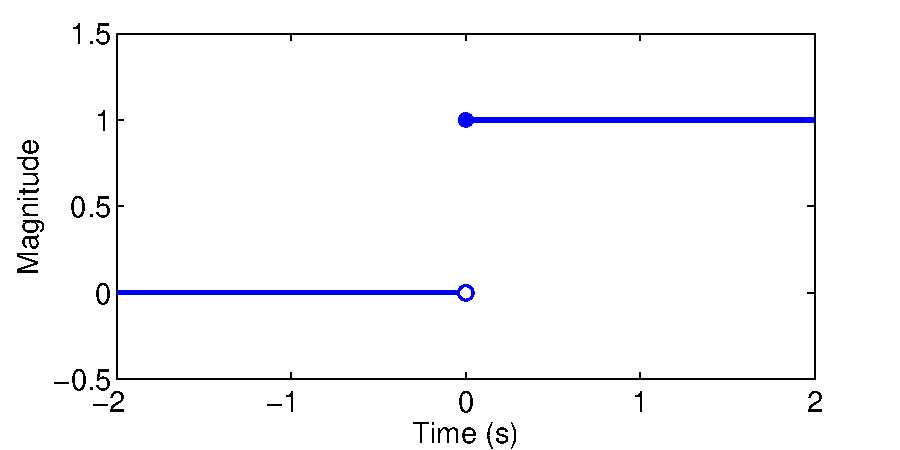
\includegraphics[width=2.4in]{figures/step}
\end{minipage}
\end{frame}

The unit step function is a signal we'll see very commonly as an input to systems in this course, as illustrated by the figure below for a generic system.
\begin{frame}
	\begin{center}
		\input{figures/unitstepsignal.tex}
	\end{center}
\end{frame}


\begin{frame}{Our First Laplace Transform Pair}
\[
3\step(t)  \overset{\mathcal{L}}{\longleftrightarrow} \frac{3}{s}
\]
where $\step(t)$ is the unit step function\vspace{.1in}\\<all>
\end{frame}

\begin{example} 
Find the Laplace Transform of the function
\[
f(t)=  Ae^{-at} \step(t)
\]
where $A$ and $a$ are fixed constants.\vspace{.1in}

\textbf{Solution: } Plug the function into the Laplace Transform definition
\begin{align*}
F(s) &= \int_{0^{-}}^{\infty} Ae^{-at}e^{-st}dt \\
&= \int_{0^{-}}^{\infty} Ae^{-(a+s)t}dt \\
& = \left.\frac{A}{-(a+s)}e^{-(a+s)t}\right|_{0^{-}}^{\infty}\\
& = \frac{A}{-(a+s)}\left[e^{-(a+s)\infty} - e^{-(a+s)0} \right] \\
& = \frac{A}{-(a+s)}\left[0 -1 \right] \\
& = \frac{A}{(a+s)} \\
\end{align*}
\end{example}

\begin{frame}{Second Laplace Transform Pair}
\[
Ae^{-at}\step(t)  \overset{\mathcal{L}}{\longleftrightarrow} \frac{A}{a+s}
\]
\end{frame}

%\begin{frame}{Example 3}
%Find the Laplace Transform of the function
%\[
%f(t)= \begin{cases} 1 &  0 \leq t \leq 2 \\
%0 & \mbox{otherwise}
%\end{cases}
%\]
%where $a$ is a fixed constant.
%\end{frame}\\
%\textbf{Solution: } Plug the function into the Laplace Transform definition
%\begin{align*}
%F(s) &= \int_{0^{-}}^{2} e^{-st}dt \\
%& =\left. \frac{1}{-s}e^{-st}\right|_{0^{-}}^{2} \\
%& = \frac{1}{-s}\left[e^{-2s} - 1\right] \\
%& = \frac{1-e^{-2s}}{s}
%\end{align*}

\section{Laplace Transform Properties}

The Laplace Transform has useful properties that can help us find the Laplace Transform of more complicated functions.

\subsection{Scaling and Linearity}

The scaling and linearity properties of the Laplace Transform are inherited from the linearity of the integral defining the Laplace Transform. Remember, we are using the notation $\mathcal{L}\{f(t)\}$ to indicate the Laplace Transform of $f(t)$.

\begin{frame}
\begin{description}
\item[Scaling] $\mathcal{L}\{Af(t)\}=A\mathcal{L}\{f(t)\}$

\item[Linearity] $\mathcal{L}\{f(t)+g(t)\}=\mathcal{L}\{f(t)\}+\mathcal{L}%
\{g(t)\}$
\end{description}
\end{frame}

A useful application of the linearity property is to find the Laplace
Transform of $\cos (\omega t) \step(t)$ from the sum of complex exponentials
\begin{example}
Using Euler's formula, $\cos (\omega t) \step(t)$ can be represented as the sum of complex exponentials 
\begin{equation*}
\cos (\omega t) \step(t)=\frac{1}{2}\left( e^{j\omega t}+e^{-j\omega t}\right)\step(t).
\end{equation*}
Using the linearity and scaling properties, the Laplace transform of a cosine is the sum of the Laplace transform of the complex exponentials, so that 
\begin{equation*}
\mathcal{L}\{\cos (\omega t) \step(t)\}=\frac{1}{2}\mathcal{L}\{e^{j\omega t}\step(t)\}+\frac{1%
}{2}\mathcal{L}\{e^{-j\omega t}\step(t)\}.
\end{equation*}
We have already derived the Laplace Transform pair
\[
e^{-at}\step(t)  \overset{\mathcal{L}}{\longleftrightarrow} \frac{1}{a+s}.
\]
Using this, we have 
\begin{eqnarray*}
\mathcal{L}\{\cos (\omega t) \step(t)\} &=&\frac{1}{2}\frac{1}{s-j\omega }+\frac{1}{2}%
\frac{1}{s+j\omega}, \\
&=&\frac{s}{s^{2}+\omega ^{2}}.
\end{eqnarray*}
\qed
\end{example}

By subtracting two complex exponentials, the same method can be used to find the Laplace Transform of sine
\begin{frame}{Sine and Cosine Laplace Transform Pair}
\begin{align*}
\cos (\omega t) \step(t) &\overset{\mathcal{L}}{\longleftrightarrow} \frac{s}{s^{2}+\omega ^{2}}\\
\sin (\omega t) \step(t) &\overset{\mathcal{L}}{\longleftrightarrow} \frac{\omega}{s^{2}+\omega ^{2}}
\end{align*}
\end{frame}

\subsection{Time and frequency shift}

A common occurrence in control systems is for a signal to be delayed due to transmission delays or other effects. When a signal is delayed, this has the effect of shifting the signal in time. To model this effect, we can use the time shift theorem given below.   Many Laplace
Transform rules have a ``dual'' form with symmetry between the time domain
and transform domain, and we list the dual to the time shift property here,
which is called the frequency shift property. In these definitions $F(s)=\mathcal{L}\left\{ f(t)\right\}$.

\begin{frame}
\begin{description}
\item[Time shift] $\mathcal{L}\left\{ f(t-t_{0})\step(t-t_{0})\right\}
=e^{-st_{0}}F(s)$

\item[Frequency shift] $\mathcal{L}\left\{ e^{-s_{0}t}f(t)\right\}
=F(s+s_{0})$
\end{description}
\end{frame}

%When applying the time shift property, it is critical to include the unit
%step function, and to make sure that the template above is followed exactly.
%
%\begin{example}
%Find the Laplace Transform of the signal 
%\begin{equation*}
%f(t)=\left\{ 
%\begin{array}{cc}
%1 & 0<t<T \\ 
%0 & \mbox{otherwise}%
%\end{array}
%\right.
%\end{equation*}
%
%Solution: We can represent this signal as the difference of two step functions: 
%\begin{equation*}
%f(t)= \step(t) -  \steparg{t-T}
%\end{equation*}
%Using the time shift property, we can find the Laplace Transform as
%\begin{equation*}
%F(s)=\frac{1}{s}-\frac{e^{-sT}}{s}
%\end{equation*}
%\qed
%\end{example}

\begin{example}
Use the frequency shift property to find the Laplace Transform of a decaying exponential function
$[g(t) = e^{-at}\cos(\omega t)\step(t)]$
%\tryit{
%\begin{boxedminipage}{6.5 in}
%\rule{0pt}{12pt}\vspace{2in}
%\color{lightgray}
%\[ 
%\mathcal{L}\{e^{-at}\cos(\omega t) \step(t) \}=\frac{s+a}{(s+a)^{2}+\omega ^{2}}
%\]
%\end{boxedminipage}\\
%}{
%\begin{boxedminipage}{6.5in}
\textbf{Solution:} Since
\[ 
\cos (\omega t) \step(t) \overset{\mathcal{L}}{\longleftrightarrow} \frac{s}{s^{2}+\omega ^{2}} 
\]
the frequency shift property implies,
\begin{align*}
\mathcal{L}\{e^{-at}\cos(\omega t) \step(t) \} &= \left.\frac{s}{s^{2}+\omega ^{2}}\right|_{s=s+a}, \\
& = \frac{s+a}{(s+a)^{2}+\omega ^{2}}.
\end{align*}
%\end{boxedminipage}
%}
%\end{frame}
\end{example}
The same method can be used to show
\begin{align*}
\mathcal{L}\{e^{-at}\sin(\omega t) \step(t) \}  = \frac{\omega}{(s+a)^{2}+\omega ^{2}}.
\end{align*}

%\subsection{Time scaling}
%
%Sometimes it is useful to change the time scale of a known function to
%create a new one
%
%\begin{description}
%\item[Time scaling] $\mathcal{L}\left\{ f(ct)\right\} =\frac{1}{c}F(\frac{s}{%
%c})$
%\end{description}
%
%where $c$ is a constant.
%
\subsection{Differentiation and Integration}
Taking the derivative of a function is equivalent in the Laplace domain to
multiplying by $s$. This property will be important when solving
differential equations. 

\begin{frame}
\begin{description}
\item[Differentiation] $\mathcal{L}\left\{ \frac{d}{dt}f(t)\right\} =s%
\mathcal{L}\left\{ f(t)\right\} -f(0^{-})$

\item[Integration] $\mathcal{L}\left\{ \int_{0}^{t}f(\tau )d\tau \right\} =%
\frac{1}{s}\mathcal{L}\left\{ f(t)\right\} $
%\item[$t-$multiplication] $\mathcal{L}\left\{ tf(t)\right\} =-\frac{d}{ds}%
%F(s)$
\end{description}
\end{frame}

Remember, the notation $f(0^{-})$ indicates the limit as we approach 0 from the left, or
\[
f(0^{-}) = \lim_{t \rightarrow 0,\; t<0} f(t).
\]
The proof of these theorems is actually pretty easy - see the appendix for the differentiation theorem. The differentiation theorem will be used in the next lecture to solve differential equations.

\begin{example} (using Integration theorem.) Find the Laplace Transform of the function $f(t)=t\step(t)$. \vspace{.1in}\\
\textbf{Solution:} We can use the integration formula because a ramp is the integral of a step. That is, 
\[
\int_{0^{-}}^{t} \steparg{\tau}d\tau = t \step(t).
\]
Thus,
\begin{align*}
\mathcal{L}\left\{t\step(t)\right\}& = \frac{1}{s}\mathcal{L}\left\{\step(t)\right\}, \\
& = \frac{1}{s}\frac{1}{s} = \frac{1}{s^{2}}. 
\end{align*}
\qed

In terms of our input and output signal and system block/arrow representation, we can visualize this example in the time domain as
\begin{frame}
	\begin{center}
		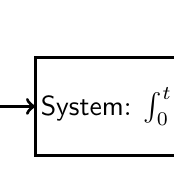
\begin{tikzpicture}[inner sep=0pt,outer sep=0pt,very thick,
sysblock/.style={draw,rectangle,inner sep=2pt,minimum width=1.5cm,minimum height=1.25cm,very thick}]
\useasboundingbox (-1,1) rectangle (0.5,-0.5); 
\begin{scope}[transform canvas={scale=1}]
\draw (0,0) node[sysblock] (S) {\textsf{System}: $\int_{0}^{t}$};
\draw[->] (-3,0) node[above=2pt] {\textsf{Input}: $u(t)$} -- (S.180);
\draw[->] (S.0) -- ++(2,0) node[above=2pt] {\textsf{Output}: $tu(t)$};
\end{scope}
\end{tikzpicture}

	\end{center}
\end{frame}
\noindent or in the Laplace domain as
\begin{frame}
	\begin{center}
		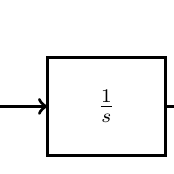
\begin{tikzpicture}[inner sep=0pt,outer sep=0pt,very thick,
sysblock/.style={draw,rectangle,inner sep=2pt,minimum width=1.5cm,minimum height=1.25cm,very thick}]
\useasboundingbox (-1,1) rectangle (0.5,-0.5); 
\begin{scope}[transform canvas={scale=1}]
\draw (0,0) node[sysblock] (S) {$\frac{1}{s}$};
\draw[->] (-2,0) node[above=2pt] {\textsf{Input}: $\frac{1}{s}$} -- (S.180);
\draw[->] (S.0) -- ++(2,0) node[above=2pt] {\textsf{Output}: $\frac{1}{s^2}$};
\end{scope}
\end{tikzpicture}

	\end{center}
\end{frame}
\noindent Note that signals and systems can be difficult to distinguish in the Laplace domain. In this unit step + integrator example, both the input signal and the system are $\frac{1}{s}$. 
\end{example}

%
%\subsection{Convolution}
%
%Convolution in the time domain is equivalent to multiplication in the
%Laplace domain, a fact we will examine more later
%
%\begin{description}
%\item[Convolution] $\mathcal{L}\left\{ \int_{0}^{t}f_{1}(t-\tau )f_{2}(\tau
%)d\tau \right\} =F_{1}(s)F_{2}(s)$
%\end{description}

%\subsection{Initial and final value theorems}
%
%The final value theorem is used extensively in control system design and
%should be committed to memory or marked for easy reference, and we will be
%using it several times throughout the semester. This results hold if $f(t)$
%and $\frac{df}{dt}$ are Laplace transformable
%
%\begin{description}
%\item[Initital value theorem] $f(0^{+})=\lim\limits_{s\rightarrow \infty
%}sF(s)$ (if $\lim\limits_{s\rightarrow \infty }sF(s)$ exists) (Note $0^{+}$ -%
%see $\frac{1}{s}$ as an example)
%
%\item[Final value theorem] $f(\infty )=\lim\limits_{s\rightarrow 0}sF(s)$
%(if $\lim\limits_{t\rightarrow \infty }f(t)$ exits or if $sF(s)$ has no
%poles in the closed RHP)
%\end{description}
%
%\begin{example}
%Find the limit as time goes to infinity of the function whose Laplace
%transform is 
%\begin{equation*}
%F(s)=\frac{s+1}{s\left( s+2\right) }
%\end{equation*}
%
%\textbf{Solution: }By the final value theorem, 
%\begin{eqnarray*}
%\lim_{t\rightarrow \infty }f(\infty ) &=&\lim_{s\rightarrow 0}s\frac{s+1}{%
%s\left( s+2\right) } \\
%&=&\frac{1}{2}
%\end{eqnarray*}
%we found earlier that this was the Laplace transform of 
%\begin{equation*}
%f(t)=\left( .5+.5e^{-2t}\right) 1(t)
%\end{equation*}
%so the result matches what we expect.
%\end{example}



\section{The Impulse Function}

A useful yet tricky signal that finds a lot of use in control systems is the impulse function. It is an
approximation to a signal which lasts for a short period of time - much
shorter than the natural time scales of the system. It turns out that the Laplace Transform of an impulse function is very simple.
However, before looking at an
\textit{im}pulse function, first let's consider a pulse with a width that we can define:

\begin{example}
Find the Laplace Transform of the pulse function
\begin{frame}{Definition of pulse function} 
\begin{equation*}
p_{t_{0}}(t)=\left\{ 
\begin{array}{cc}
\frac{1}{t_{0}} & 0<t<t_{0} \\ 
0 & \mbox{otherwise}%
\end{array}
\right.
\end{equation*}
where $t_{0}$ is a constant. 
\begin{center}
\includegraphics[width=3in]{figures/pulse}
\end{center}
\end{frame}
Note that the area of the pulse function is $1$ for any value of $t_{0}$. 

\textbf{Solution:} The pulse function can be represented as a superposition
of steps 
\begin{equation*}
p_{t_{0}}(t)=\frac{1}{t_{0}}\step(t)-\frac{1}{t_{0}}\steparg{t-t_{0}}
\end{equation*}
so the Laplace Transform of $p_{t_{0}}(t)$ is 
\begin{eqnarray*}
\mathcal{L}\left\{ p_{t_{0}}(t)\right\} &=&\mathcal{L}\left\{ \frac{1}{t_{0}}%
\step(t) \right\} -\mathcal{L}\left\{ \frac{1}{t_{0}}\steparg{t-t_{0}}\right\} \\
&=&\frac{1}{t_{0}s}-\frac{1}{t_{0}s}e^{-st_{0}} \\
&=&\frac{1}{t_{0}s}\left( 1-e^{-st_{0}}\right)
\end{eqnarray*}
\qed
\end{example}

The impulse function is a pulse that gets shorter and shorter, but whose magnitude gets larger and larger, while maintaining the same area under the curve. 
\begin{frame}{Definition of impulse function}
\[
\delta(t) := \lim_{t_{0}\rightarrow 0} p_{t_{0}}(t)
\]
\begin{center}
\includegraphics[width=3in]{figures/pulsetoimpulse3}
\end{center}
\end{frame}

\begin{example}
Find the Laplace Transform of the impulse function $\delta(t)$.\vspace{.1in}\\
\textbf{Solution: }We can take the limit of the Laplace
Transform of the pulse function using L'Hopital's rule: 
\begin{eqnarray*}
\mathcal{L}\left\{ \delta(t)\right\} &=&\lim_{t_{0}\rightarrow 0}\frac{1}{t_{0}s}%
\left( 1-e^{-st_{0}}\right) \\
&=&\lim_{t_{0}\rightarrow 0}\frac{\frac{d}{dt_{0}}\left(
1-e^{-st_{0}}\right) }{\frac{d}{dt_{0}}\left( t_{0}s\right) }=\frac{s}{s}=1
\end{eqnarray*}
\qed
\end{example}

\begin{frame}{The simplest Laplace Transform pair}
\[
\delta(t) \overset{\mathcal{L}}{\longleftrightarrow} 1
\]
\end{frame}

The impulse function can also be defined via these two properties:
\begin{align*}
\delta (t) &=0\quad t\neq 0 \\
\int_{0^{-} }^{0^{+} }\delta (t)dt &=1 
\end{align*}
Any function which has these properties (including the limit of the pulse function) has Laplace Transform equal to one
\begin{align*}
\mathcal{L}\left\{ \delta (t)\right\} &=\int_{0^{-}}^{\infty }\delta
(t)e^{-st}dt \\
&=\int_{0^{-}}^{0^{+}}\delta (t)e^{-st}dt \\
&=e^{-s0}\int_{0^{-}}^{0^{+}}\delta (t)dt\\
&=1
\end{align*}

\section{Table of Laplace Transform Pairs}

Here is a table of the Laplace Transform Pairs derived in this lecture that you are expected to know.

\begin{center}
\begin{tabular}{cc}
$f(t)$ & $F(s)$\\\toprule
\rule{0pt}{1pt} $\delta(t)$ & 1 \\
\rule{0pt}{12pt}$\step(t)$ & $\frac{1}{s}$ \\
\rule{0pt}{12pt}$t\step(t)$ & $\frac{1}{s^2}$ \\
\rule{0pt}{12pt}$e^{-at}\step(t)$ & $\frac{1}{s+a}$ \\
\rule{0pt}{12pt}$\cos (\omega t) \step(t)$ & $\frac{s}{s^{2}+\omega ^{2}}$\\
\rule{0pt}{12pt}$\sin (\omega t) \step(t)$ &$\frac{\omega}{s^{2}+\omega ^{2}}$\\
\rule{0pt}{12pt}$e^{-at}\cos(\omega t) \step(t)$  &  $\frac{s+a}{(s+a)^{2}+\omega ^{2}}$\\
\rule{0pt}{12pt}$e^{-at}\sin(\omega t) \step(t)$  &  $\frac{\omega}{(s+a)^{2}+\omega ^{2}}$\\


\end{tabular}
\end{center}


\section{Lecture Highlights}
The primary takeaways from this article include
\begin{enumerate}
\setlength{\itemsep}{5pt}
\setlength{\parskip}{0pt}
\setlength{\parsep}{0pt}
\item Complex numbers can be represented in both polar and rectangular form. To understand the course material, you should be comfortable with both.
\item The Laplace transform is a powerful mathematical tool that makes feedback control design and analysis easier. 
\item Tables of Laplace transform pairs and properties can be derived from the definition. (These pairs and properties will facilitate transforming within the Laplace domain and the time domain in future lectures.)
\end{enumerate}

\section{Appendix}



\subsection{Euler's Formula}

The definition of the Laplace Transform includes the function $e^{-st}$, where $s$ is a complex number. Let's remember how to integrate this function.  The function $e^{x}$ is very important, as it appears in many places in engineering subjects. The reason that it is so ubiquitous is that it satisfies the relationship
\[
\frac{d}{dx}e^{x}=e^{x}
\]
and thus appears in situations when quantities increase in proportion to how much is already there.
We want to extend this function to complex numbers. In this case, we will need to calculate $e^{z}$ when $z$ is complex. 

\begin{itemize}
\item The key formula extending exponentials to complex numbers is Euler's Formula:
\[
\boxed{e^{j\theta}=\cos(\theta)+j\sin(\theta)}
\]
\end{itemize}

Let's check that with this definition, $e^{j\theta}$  satisfies $\frac{d}{d\theta}e^{j\theta}=je^{j\theta}$
\begin{align*}
\frac{d}{d\theta}e^{j\theta} & = \frac{d}{d\theta}\left(\cos(\theta)+j\sin(\theta)\right)\\
&= -\sin(\theta) + j\cos(\theta) \\
&= j\left(\cos(\theta) + j\sin(\theta)\right) \quad \quad \mbox{[switch terms, pull out $j$ and use $j^2=-1$]}\\
&=j e^{j\theta} 
\end{align*}

Now, considering $\frac{de^{st}}{dt}$ we can write $s=a+jb$, so that
\begin{align*}
\frac{de^{st}}{dt}&=\frac{de^{(a+jb)t}}{dt}\\
&=\frac{d(e^{at}e^{jbt})}{dt}\\
&= ae^{at}e^{jbt}+jbe^{at}e^{jbt}\\
& = (a+jb)e^{at}e^{jbt}\\
& = se^{st}
\end{align*}
Thus, taking the derivative of $e^{st}$ with respect to time simply brings down the factor $s$, just as would occur if $s$ were purely real. This also means that 
\[
\int_{a}^{b} e^{st}dt = \left.\frac{1}{s}e^{st}\right|_{a}^{b}
\]

\subsection{Proof of Time Shift Property}
\begin{align*}
\mathcal{L}\left\{ f(t-t_{0})\step(t-t_{0})\right\} & = \int_{0^{-}}^{\infty} f(t-t_{0})\step(t-t_{0})e^{-st}dt\\
 & = \int_{t_{0}^{-}}^{\infty} f(t-t_{0})e^{-st}dt\\
 & = \int_{{0}^{-}}^{\infty} f(\tau)e^{-s(\tau+t_{0})}d\tau \quad \mbox{[change of variable $\tau=t-t_{0}$]}\\
 & = e^{-st_{0}}\int_{{0}^{-}}^{\infty} f(\tau)e^{-s(\tau)}d\tau \\
 & = e^{-st_{0}}F(s)
\end{align*}

\subsection{Proof of Frequency Shift Property}
\begin{align*}
\mathcal{L}\left\{ e^{-s_{0}t}f(t)\right\} & = \int_{0^{-}}^{\infty} f(t)e^{-s_{0}t}e^{-st}dt\\
& = \int_{0^{-}}^{\infty} f(t)e^{-(s_{0}+s)t}dt\\
& = \left.F(s)\right|_{s\leftarrow s+s_{0}}
\end{align*}

\subsection{Proof of Differentiation Theorem}
\begin{equation*}
\mathcal{L}\left\{ \frac{d}{dt}f(t)\right\} =\int_{0^{-}}^{\infty }\frac{%
df(t)}{dt}e^{-st}dt
\end{equation*}%
Choose $u=e^{-st}$ and $dv=\frac{df(t)}{dt}dt.$ Then $du=-se^{-st}dt$ and $%
v=f(t)$ so that%
\begin{align*}
\mathcal{L}\left\{ \frac{d}{dt}f(t)\right\} &=\left. f(t)e^{-st}\right\vert
_{0^{-}}^{\infty }+\int_{0^{-}}^{\infty }f(t)se^{-st}dt \\
&=\lim_{t\rightarrow \infty }\cancelto{\tiny 0}{f(t)e^{-st}} \quad
-f(0^{-})+s\int_{0^{-}}^{\infty }f(t)e^{-st}dt \\
&=s\mathcal{L}\left\{ f(t)\right\} -f(0^{-})
\end{align*}

\subsection{Proof of Integration Theorem}
\begin{align*}
\mathcal{L}\left\{ \int_{0}^{t}f(\tau)d\tau\right\} &=\int_{0^{-}}^{\infty }\int_{0}^{t}f(\tau)e^{-st}d\tau dt
\end{align*}%
Choose $u=\int_{0}^{t}f(\tau)d\tau$ and $dv=e^{-st}$. Then $du=f(t)$ and $v=\frac{1}{s}e^{-st}$ so that
\begin{align*}
\mathcal{L}\left\{ \int_{0}^{t}f(\tau)d\tau\right\} &= \left.\int_{0}^{t}f(\tau)d\tau\frac{1}{s}e^{-st}\right|_{0^{-}}^{\infty} + \int_{0^{-}}^{\infty }f(t)\frac{1}{s}e^{-st}dt \\
& = \lim_{t\rightarrow\infty} \cancelto{\tiny 0}{\int_{0}^{t}f(\tau)d\tau\frac{1}{s}e^{-st}} - \cancelto{\tiny 0}{\int_{0}^{0}f(\tau)d\tau\frac{1}{s}e^{0}} + \frac{1}{s}\int_{0^{-}}^{\infty }f(t)e^{-st}dt\\
& = \frac{1}{s}\mathcal{L}\{f(t)\}
\end{align*}%
Note that the above proof assumes that as $t \rightarrow \infty$, $f(t)$ can be bounded by $e^{\alpha t}$ for some $\alpha$. 
\section{Quiz Yourself}

\subsection{Questions}


\begin{enumerate}
\setlength{\itemsep}{5pt}
\setlength{\parskip}{0pt}
\setlength{\parsep}{0pt}
\item Find the one-sided Laplace Transform for the following signals
\begin{enumerate}
\setlength{\itemsep}{5pt}
\setlength{\parskip}{0pt}
\setlength{\parsep}{0pt}
\item $x(t)=\begin{cases} 1 & 0 \leq t \leq 1 \\ 0 & \text{otherwise} \end{cases}$ 
\item $x(t)=(1+e^{-t})$
\item $x(t)=(1+e^{-t})\step(t)$
\item $x(t)=t$
\end{enumerate}
\item Using the step function and the integration formula, find the Laplace Transform of the following function
\[
x(t) = t^{2}\step(t)
\]
\item Using the frequency shift property, find the Laplace Transform of the following function
\[
x(t) = e^{-t}t^{2}\step(t)
\]
\end{enumerate}

\subsection{Solutions}
\begin{enumerate}
\setlength{\itemsep}{5pt}
\setlength{\parskip}{0pt}
\setlength{\parsep}{0pt}
\item \rule{0pt}{12pt}\\
\begin{enumerate}
\setlength{\itemsep}{5pt}
\setlength{\parskip}{0pt}
\setlength{\parsep}{0pt}
\item\rule{0pt}{12pt}\\
\begin{center}
\includegraphics[width=4in]{quizfigures/1asoln}
\end{center}
\item\rule{0pt}{12pt}\\
\begin{center}
\includegraphics[width=4in]{quizfigures/1bsoln}
\end{center}\pagebreak
\item\rule{0pt}{12pt}\\
\begin{center}
\includegraphics[width=4in]{quizfigures/1csoln}
\end{center}
\item\rule{0pt}{12pt}\\
\begin{center}
\includegraphics[width=4in]{quizfigures/1dsoln}
\end{center}
\end{enumerate}\pagebreak
\item \rule{0pt}{12pt}\\
\begin{center}
\includegraphics[width=4in]{quizfigures2/1soln}
\end{center}
\item\rule{0pt}{12pt}\\
\begin{center}
\includegraphics[width=4in]{quizfigures2/2soln}
\end{center}

\end{enumerate}


\section{Resources}

\subsection{Books}
Laplace Transforms are often covered in textbooks on differential equations or advanced engineering  math. A Laplace Transform review is also often part of an introductory controls textbook. The following is a small subset of relevant books.

\begin{itemize}
\item Norman S. Nise, {\em Control Systems Engineering}, Wiley
\begin{itemize}
\item 7th edition: Section 2.2
\end{itemize}
\item Richard C. Dorf and Robert H. Bishop, {\em Modern Control Systems}, Pearson
\begin{itemize}
\item 13th edition: Section 2.4
\end{itemize}
\item Gene F. Franklin, J. David Powell and Abbas Emami-Naeini,  {\em Feedback Control of Dynamic Systems}, Pearson
\begin{itemize}
\item 6th and 7th edition: Section 3.1
\end{itemize}
\item Erwin Kreyszig, {\em Advanced Engineering Mathematics}, Wiley
\begin{itemize}
\item 10th edition: Section 6.1, 6.3, 6.4
\end{itemize}

\end{itemize}

\subsection{Web resources}
There are also some web resources that cover Laplace Transforms. If you find something useful, or if you find a link that no longer works, please inform your instructor!

\begin{itemize}
\item There are lots and lots of videos on Laplace Transforms.
\begin{itemize}
\item From the Khan Academy an \href{https://www.khanacademy.org/math/differential-equations/laplace-transform/laplace-transform-tutorial/v/laplace-transform-1}{introduction} and  \href{https://www.khanacademy.org/math/differential-equations/laplace-transform/properties-of-laplace-transform/v/laplace-transform-5}{discussion of Laplace Transform Properties}. 
\item From \href{http://ocw.mit.edu/courses/mathematics/18-03-differential-equations-spring-2010/video-lectures/lecture-19-introduction-to-the-laplace-transform/}{MIT open courseware}. A 50 minute lecture on Laplace Transforms for those that like things old school.
\end{itemize}
\end{itemize}


\end{document}


